% §3 System - ~1 page (~600 words) including Fig 1. v0 draft.
\label{sec:system}

A.L.F.R.E.D.\ sits between a user-facing chat surface and a set of skill backends invoked via command-line tools (Fig.~\ref{fig:arch}). A single user message flows through three components: the \emph{Pattern Store}, the \emph{Router}, and one of two execution tiers (\emph{Reflexer} or \emph{Thinker}) before reaching the skill backends.

\begin{figure}[t]
  \centering
  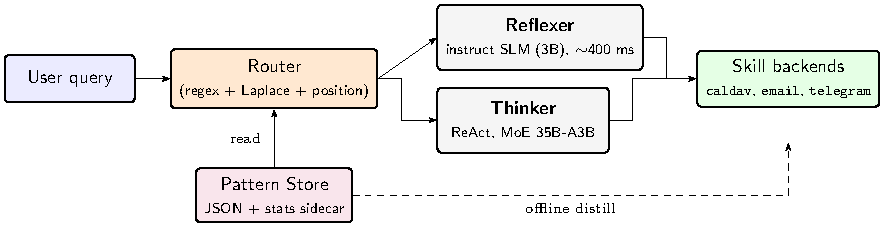
\includegraphics[width=\columnwidth]{figures/fig1_architecture.pdf}
  \caption{A.L.F.R.E.D.\ architecture. The Router scores active patterns against the user query and selects the cheaper applicable tier. The Reflexer is a small instruction-tuned LLM given only the matched pattern's compressed slice; the Thinker is a full-context ReAct loop retained as fallback. The Pattern Store is read by the Router and updated offline by a distiller.}
  \label{fig:arch}
\end{figure}

\textbf{Patterns.} A pattern is a typed JSON record carrying (a) one or more \emph{trigger} regular expressions, (b) a \emph{slot schema} naming string-, date-, and integer-typed parameters with type validators, (c) a \emph{command template} with literal arguments and slot references, and (d) a \emph{status} marker (\texttt{active} or \texttt{draft}). Patterns are produced offline from a SKILL.md~\cite{anthropic2025skills} file by a distiller. A separate stats sidecar records per-pattern use counts, success counts, and last-use timestamps.

\textbf{Router.} On each query the Router computes a score for every active pattern whose trigger matches the query:
\[
  s(p) = 0.6\,\mathrm{succ}(p) + 0.2\,\mathrm{rec}(p) + 0.2\,\mathrm{spec}(p) + b_{\text{pos}}(p),
\]
where $\mathrm{succ}(p)$ is the Laplace-smoothed success rate $(s+1)/(n+2)$ with a cold-start prior of $0.8$ when $n=0$, $\mathrm{rec}(p)$ is a recency decay over last-used timestamp, $\mathrm{spec}(p)$ penalises overly generic triggers, and $b_{\text{pos}}=0.15$ is a bonus awarded when the trigger matches in the first 50 characters of the query. The top pattern wins; if the score margin to the runner-up falls below $0.05$, the Router emits an \emph{ambiguous} verdict and defers to the Reflexer for a one-call disambiguation.

\textbf{Reflexer.} When the Router selects a pattern above the confidence threshold, A.L.F.R.E.D.\ invokes the Reflexer: a small instruction-tuned LLM (Ministral-3-3B-Instruct~\cite{ministral2025} in our experiments) prompted with only the matched pattern's compressed slice (trigger, schema, template, examples) and the user query. The Reflexer always emits the final executable command; any slot values captured by the trigger regex are passed to it as hints rather than bypassing it. The name draws a deliberate analogy to the biological reflex arc, in which a stimulus triggers a fast motor response routed through the spinal cord without engaging higher cortical deliberation~\cite{sherrington1906}; in dual-process terms~\cite{kahneman2011}, the Reflexer is the System~1 path (fast, automatic, pattern-cued) and the Thinker is the System~2 path (slow, deliberate). The Reflexer is not to be confused with Reflexion~\cite{shinn2023reflexion}, a self-reflective revision loop.

\textbf{Thinker.} When the Router finds no pattern above threshold, the query escalates to a ReAct~\cite{yao2022react} agent (Qwen3.6-35B-A3B~\cite{qwen3_6} in our experiments) with full SKILL.md context. This tier is the safety net: it preserves correctness on out-of-distribution queries at the cost of higher latency and full-model token spend.
